\begin{figure*}[t]
\centering
  \begin{subfigure}[b]{0.33\textwidth}
    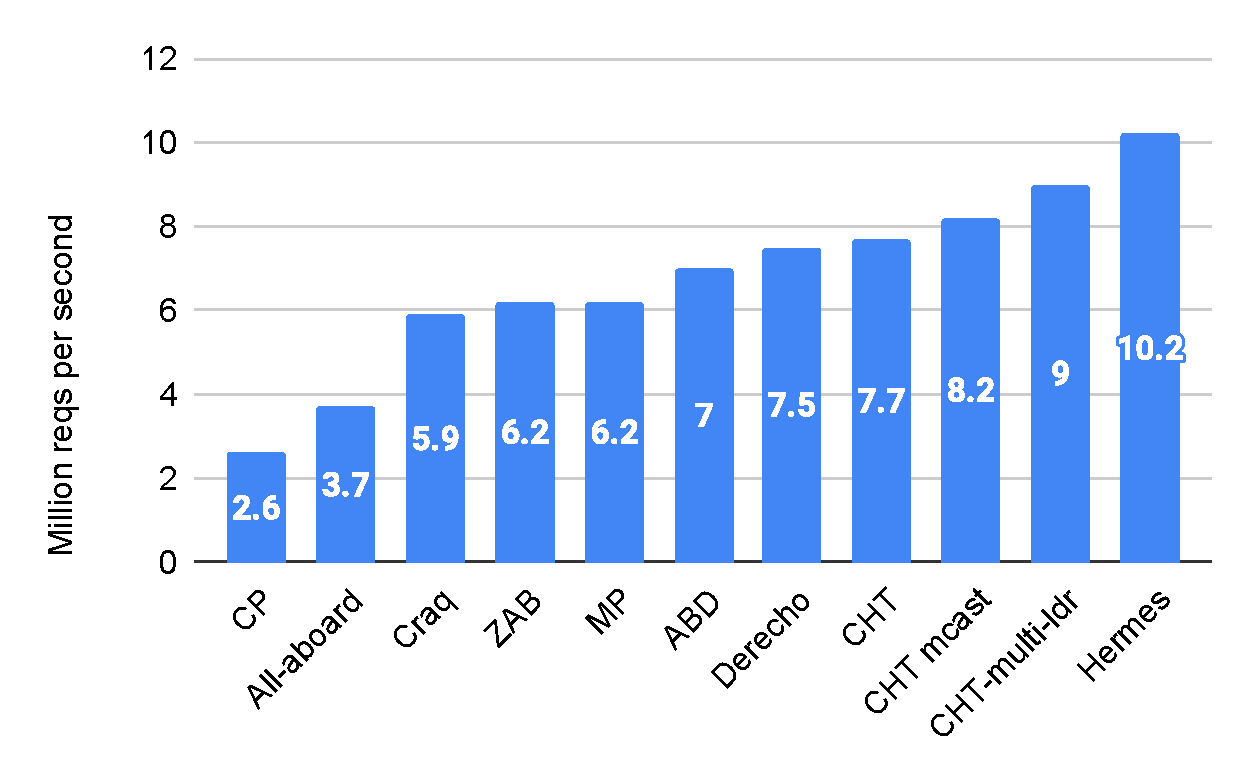
\includegraphics[width=\textwidth]{1_figures/single-thread.pdf}
    % \captionsetup{width=0.85\linewidth}
    % \vspace{-1.8em}
    \caption{Single-threaded write throughput}
%   \vspace{-1.5em}
  \label{fig:single-thr}
  \end{subfigure}
  %
  \begin{subfigure}[b]{0.33\textwidth}
    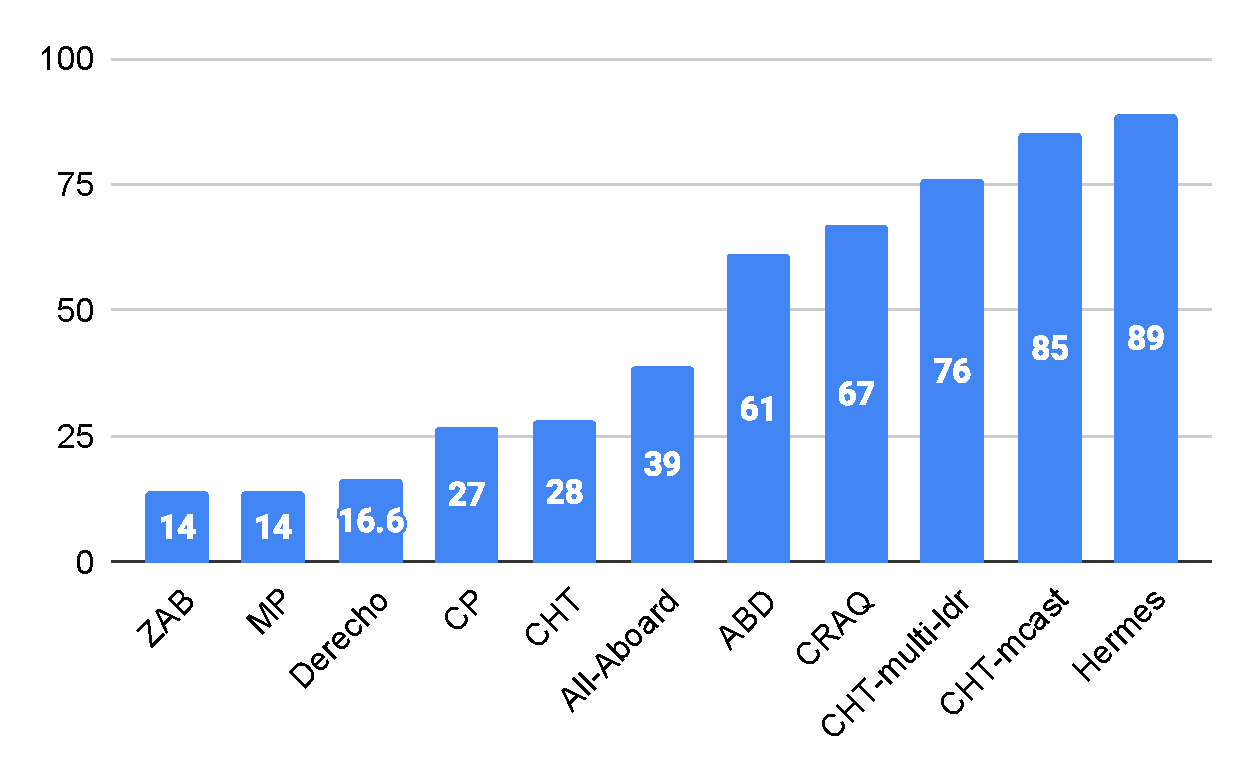
\includegraphics[width=\textwidth]{1_figures/Write-only-chart.pdf}
    % \captionsetup{width=0.85\linewidth}
    % \vspace{-1.8em}
    \caption{Multi-threaded write throughput}
    %   \vspace{-1.5em}
  \label{fig:write-all}
  \end{subfigure}
  %
  \begin{subfigure}[b]{0.33\textwidth} 
  
    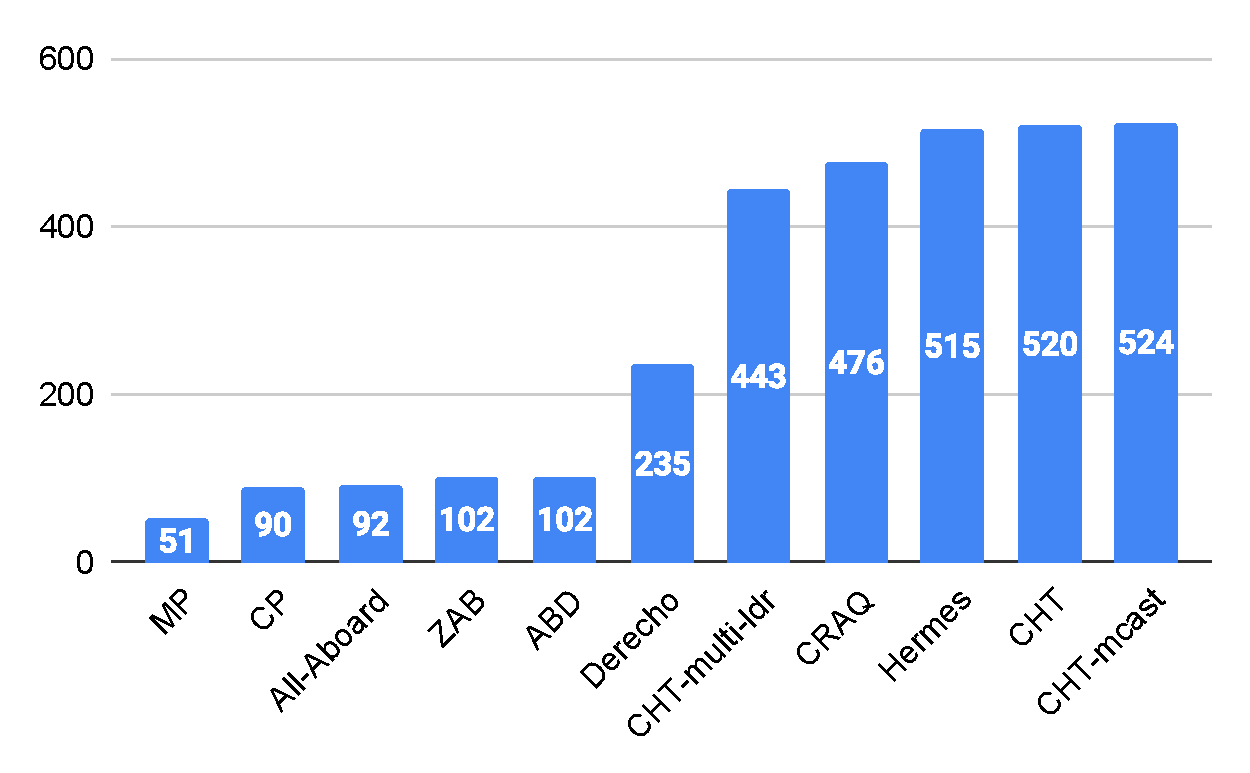
\includegraphics[width=\textwidth]{1_figures/5perc-writes.pdf}
    % \captionsetup{width=0.85\linewidth}
    % \vspace{-1.8em}
    \caption{Multi-threaded throughput at 95\% reads}
%   \vspace{-1.5em}
  \label{fig:5perc}
  \end{subfigure}
%   \vspace{-1em}
  \caption{Throughput comparison of all protocols in M.reqs/s. Note that both the x-axes and y-axes are different in each graph.}
 %\antonis{caption is closer to the text below than the subcaptions above}}
  \label{fig:three-bars}
%   \vspace{-1em}
\end{figure*}